The first part of this chapter will discuss results of calculations with each of the decusping methods implemented in MPACT.  We will see which of them is best and how much room there is for improvement.  The second part of the chapter will discuss the results of some tests performed with a 1D MOC code.  These results will focus primarily on the effects that partially inserted rods have on the angular flux, rather than applying corrections to the cross-sections or scalar fluxes at the end of a calculation.

\section{MPACT Decusping Results}

To test MPACT's decusping methods, VERA Progression Problem 4 \cite{VERAProgressionProblems} was used.  This problem is composed of a 3x3 set of assemblies, with an AIC control bank in the center assembly.  The radial layout of the problem is shown in figure \ref{f:p4radial}, and the axial layout of each assembly is shown in figure \ref{f:p4axial}.  The control rods were placed at an axial elevation of \hl{numbers} above the core plate. \hl{Note about hybrid rod}

For the reference solution, 58 MOC planes were used.  It was also ensured that the end of the control rods were exactly aligned with one of the MOC plane boundaries.  The cases using decusping methods used the same mesh, but with the 2 MOC planes around the tip of the control rod merged into a single plane to introduce cusping effects.  The accuracy and convergence data for these cases are shown in table \ref{t:p4decusp}

\begin{figure}\label{f:p4layout}
\centering
\subfigure{\label{f:p4radial}
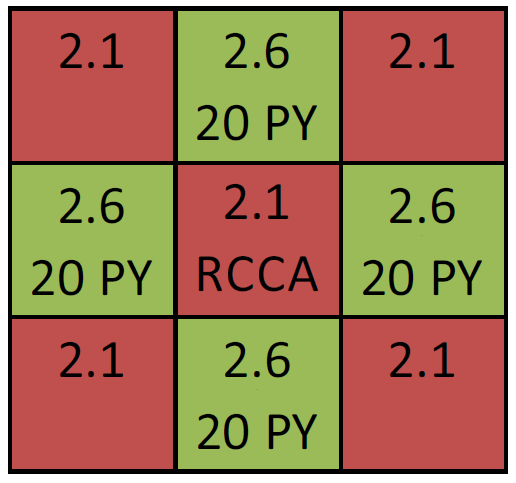
\includegraphics[width=0.4\textwidth]{figs/p4a_layout.png}
}
~
\subfigure{\label{f:p4axial}
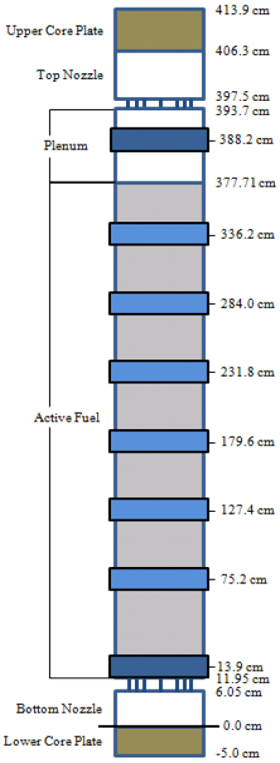
\includegraphics[width=0.4\textwidth]{figs/wb_3d_assembly.png}
}
\caption{VERA Problem 4 radial (a) and axial (b) layouts}\label{f:p4}
\end{figure}

\begin{table}
\centering
\caption{VERA Problem 4 Decusping Results}\label{t:p4decusp}
\subtable{
\begin{tabular}{|c|c|c|c|}\hline
\multirow{2}{*}{Case} & k-eff & \multicolumn{2}{|c|}{Pin Power Differences} \\\cline{3-4}
 & Difference (pcm) & RMS & Max \\\hline
Reference &  &  &  \\\hline
No Treatment &  &  &  \\\hline
Polynomial &  &  &  \\\hline
Subplane &  &  &  \\\hline
Subplane + 1D-CP &  &  &  \\\hline
\end{tabular}
}
\subtable{
\begin{tabular}{|c|c|c|c|}\hline
Case & 2D/1D Iterations & CMFD Iterations & Runtime (Core-Hours) \\\hline
Reference &  &  &  \\\hline
No Treatment &  &  &  \\\hline
Polynomial &  &  &  \\\hline
Subplane &  &  &  \\\hline
Subplane + 1D-CP &  &  &  \\\hline
\end{tabular}
}
\end{table}

\hl{Discussion}

To demonstrate the behavior of the decusping methods on a full-core problem, VERA Problem 5 was also run\todo{citation}.  Problem 5 is the a beginning-of-cycle simulation of the Watts Bar Unit 1 PWR.  The model of this reactor uses the same axial layout shown in figure \ref{f:p4axial} with the radial layout shown in figure \ref{f:p5radial}.  For these calculations, Bank D was set to a position of \hl{numbers} while all other banks were fully withdrawn.  \hl{Note about the hybrid rod}

Like problem 4, the reference case was run with 58 planes while the decusping cases were run with 57 planes.  \hl{Mention decomposition briefly?}.  The accuracy and convergence data for these calculations is shown in table \ref{t:p5decusp}.

\begin{figure}
\centering
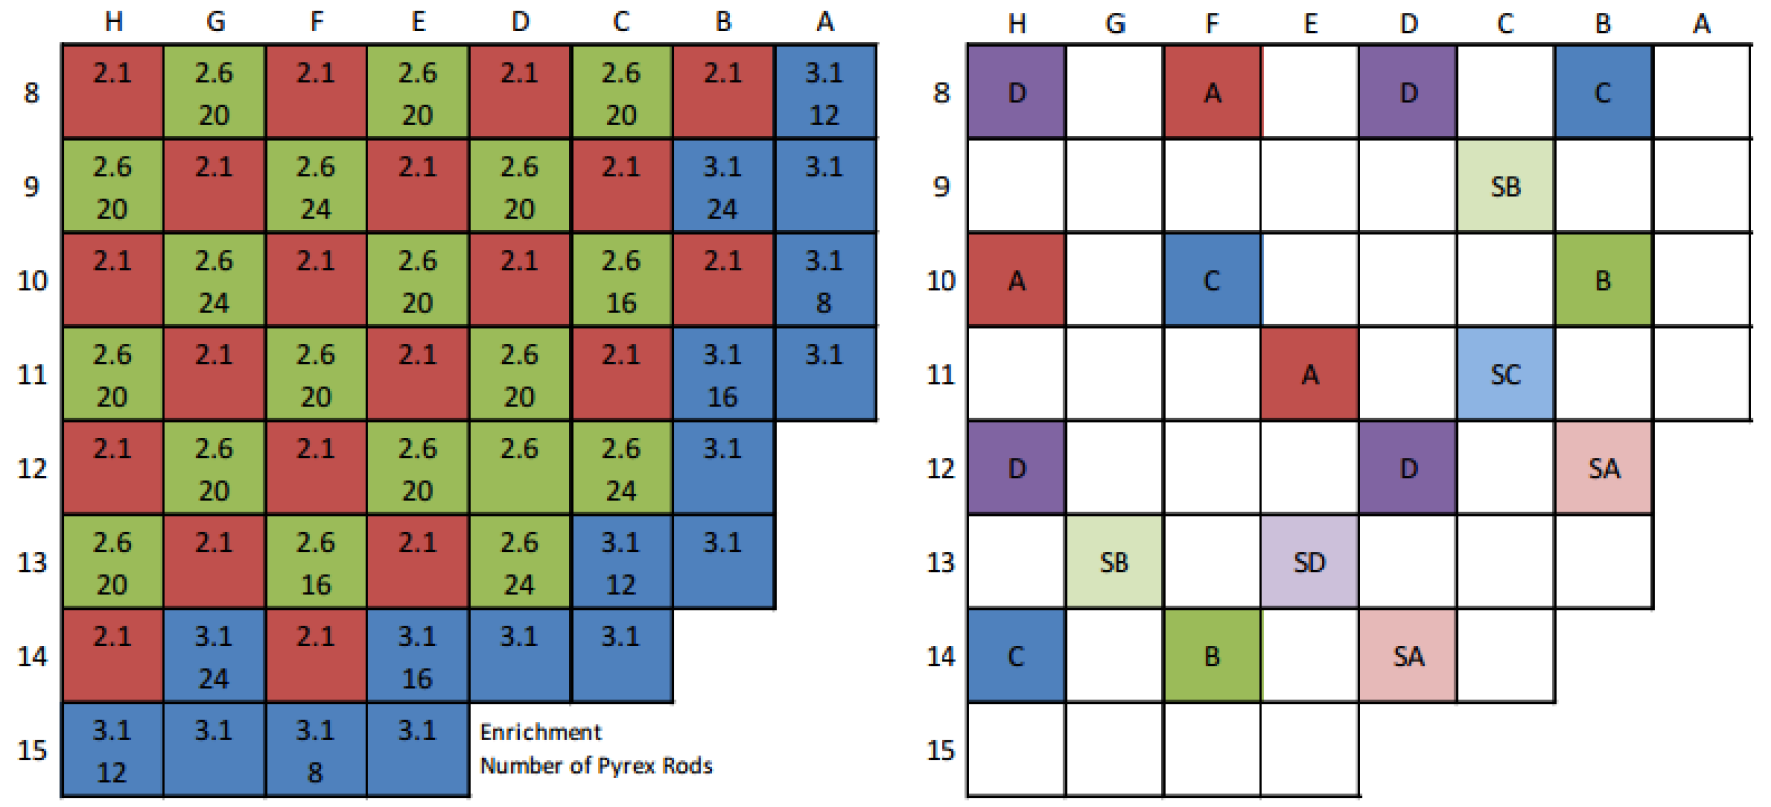
\includegraphics[width=0.9\textwidth]{figs/WB1-cycle1-layout.png}
\caption{VERA Problem 5 radial layout}\label{f:p5radial}
\end{figure}

\begin{table}
\centering
\caption{VERA Problem 4 Decusping Results}\label{t:p5decusp}
\subtable{
\begin{tabular}{|c|c|c|c|}\hline
\multirow{2}{*}{Case} & k-eff & \multicolumn{2}{|c|}{Pin Power Differences} \\\cline{3-4}
 & Difference (pcm) & RMS & Max \\\hline
Reference &  &  &  \\\hline
No Treatment &  &  &  \\\hline
Polynomial &  &  &  \\\hline
Subplane &  &  &  \\\hline
Subplane + 1D-CP &  &  &  \\\hline
\end{tabular}
}
\subtable{
\begin{tabular}{|c|c|c|c|}\hline
Case & 2D/1D Iterations & CMFD Iterations & Runtime (Core-Hours) \\\hline
Reference &  &  &  \\\hline
No Treatment &  &  &  \\\hline
Polynomial &  &  &  \\\hline
Subplane &  &  &  \\\hline
Subplane + 1D-CP &  &  &  \\\hline
\end{tabular}
}
\end{table}

\hl{discussion}

\section{1D MOC Results}

Since rod cusping is caused by an overly simplistic homogenization of two materials, a 1D MOC code was developed to analyze the impacts of rod cusping on the angular flux.  Understanding the response of the angular flux to homogenized cross-sections can then be used to develop a more effective decusping method that addresses the angular flux during the calculation instead of applying corrections to the cross-sections or scalar flux after a calculation.  This code is capable of performing both k-eigenvalue and fixed fission source calculations.  This allows the resulting fission source from a calculation to be reused in subsequent calculations to isolate the effects of the cross-section homogenization.

Two begin this analysis, VERA Problem 4 was used as a starting point.  The center row of pins across all three assemblies was modeled in 1D, creating a model that had heterogeneous representations of fuel pins, instrument tubes, and control rods.  The control rod cross-sections were then mixed with the moderator cross-sections to simulate a partially inserted control rod.  \hl{Cross-sections}

With this model set up, 